\documentclass[12pt,oneside,a4paper]{article}

\usepackage[utf8]{inputenc} % Lærer LaTeX at forstå unicode - HUSK at filen skal
% være unicode (UTF-8), standard i Linux, ikke i
% Win.

\usepackage[danish]{babel} % Så der fx står Figur og ikke Figure, Resumé og ikke
% Abstract etc. (god at have).

\usepackage{graphicx}
\usepackage{amsfonts}
\usepackage{amsthm}        % Theorems
\usepackage{amsmath}
%\usepackage{hyperref}

%\renewcommand{\mid}[1]{{\rm E}\!\left[#1\right]}
\newcommand{\bas}{\begin{eqnarray*}}
\newcommand{\eas}{\end{eqnarray*}}
\newcommand{\be}{\begin{equation}}
\newcommand{\ee}{\end{equation}}
\newcommand{\bea}{\begin{eqnarray}}
\newcommand{\eea}{\end{eqnarray}}

\newtheorem{thm}{Sætning}[section]
\newtheorem{mydef}[thm]{Definition}
\newtheorem{eks}[thm]{Eksempel}

\DeclareMathSymbol{,}{\mathord}{letters}{"3B}

\title{Linearitet}

\begin{document}

\maketitle

\section{Indledning}
Vi skal i dette afsnit beskæftige os med lineære sammenhænge mellem to variable
størrelser $x$ og $y$.  Vi begynder med at kigge på nogle eksempler.

\subsection{Eksempel (kopi af eksempel 3.1 i Mat-C bogen)}
Et teleselskab har et simpelt takstsystem:
\begin{itemize}
    \item Abonnement 20 kr. pr. måned, samt 0,50 kr. pr. talt minut.
\end{itemize}
Hvis en abonnent en måned taler 25 minutter, skal han betale:
$$
20 + 0,50\cdot25 = 32,50 \, {\rm kr},
$$
og tales der $x$ minutter en bestemt måned, er prisen $y$ kroner bestemt ved:
$$
y = 20 + 0,50\cdot x
$$
Man siger, at der er en {\em lineær sammenhæng} mellem samtaletiden og prisen.

Hvis vi afbilder sammenhængen i et koordinatsystem med antallet af minutter på
$x$-aksen og prisen på $y$-aksen, vil sammenhørende værdier af $x$ og $y$ (dvs
af taletid og pris) udgøre en ret linje med hældning $0,50$, som skærer
$y$-aksen i tallet $20$ (det koster 20 kroner at tale i 0 minutter), se figur
3.5.

\begin{figure}[ht]
    \centering
    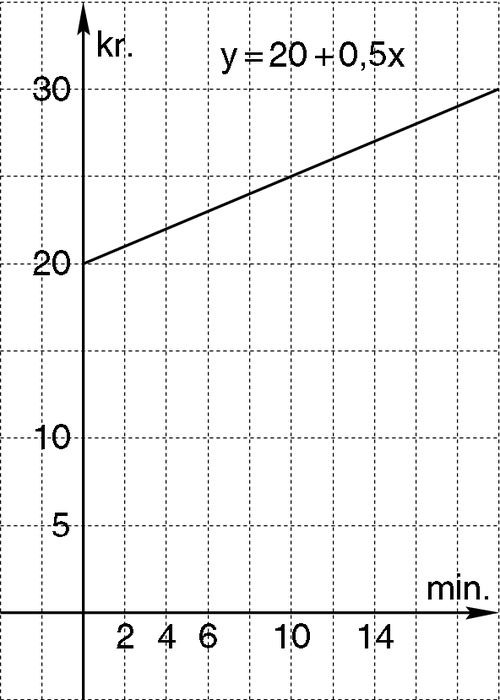
\includegraphics[width=0.5\textwidth]{fig35}
    \caption{Figur 3.5}
    \label{fig35}
\end{figure}

Hældningen $0,50$ angiver prisstigningen for hvert ekstra minut, der tales --
den er 0,50 kroner.  Prisen for 20 minutters samtale er 30 kr., og for 21
minutters samtale er den 30,50 kr.

\subsection{Eksempel -- kopi af eksempel 3.2 i Mat-C bogen}
En prøvekørsel af en bil begynder ved 5-km stenen uden for en by. Bilen kører
en længere strækning med 90 km/t. Efter 8 minutters kørsel befinder bilen sig
ved 17-km-stenen (hvorfor?), og efter $x$ minutter er den ved $y$-km-stenen,
hvor
$$
y = 5 + 1,5\cdot x
$$
Her er der tale om en lineær sammenhæng mellem tiden i minutter og tallet på
kilometerstenen.

\section{Lineære sammenhænge}
\begin{mydef}
    En variabelsammenhæng er en sammenhæng mellem en uafhængig variabel, ofte
    kaldet $x$, og en afhængig variabel, ofte kaldet $y$.
\end{mydef}

\begin{mydef}
    En lineær sammenhæng er en variabelsammenhæng givet ved følgende ligning:
    $$
    y = a\cdot x + b
    $$
    hvor $a$ og $b$ er tal.
\end{mydef}

Vi interesserer os for de koordinatsæt $(x,\,y)$, der passer i en sådan lineær
sammenhæng. Fra folkeskolen vides, at sådanne koordinatsæt udgør en ret linje.

Eksempler på sådanne lineære sammenhænge er (se figur xx):

\begin{tabular}{ll}
    $\bullet\quad y=3x-5$  & Her er $a=3$ og $b=-5$. \\
    $\bullet\quad y=-2x+1$ & Her er $a=-2$ og $b=1$. \\
    $\bullet\quad y=4-x$   & Her er $a=-1$ og $b=4$. \\
    $\bullet\quad y=3x$    & Her er $a=3$ og $b=0$.
\end{tabular}

\begin{figure}[ht]
    \centering
    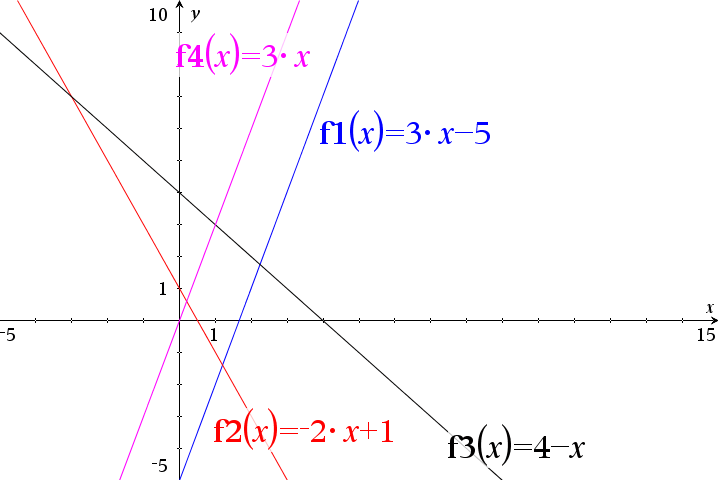
\includegraphics[width=0.5\textwidth]{fig-def-22}
    \caption{Figur xx}
    \label{fig-def-22}
\end{figure}

\begin{thm}
    For den lineære sammenhæng
    $$
    y = a\cdot x + b
    $$
    gælder, at grafen er en ret linje, hvor
    $a$ er linjens hældning, dvs linjen vokser med $a$ enheder, når
    $x$ vokser med 1 enhed. Punktet $(0,\,b)$ er linjens skæringspunkt med
    $y$-aksen.
\end{thm}

Vi kan opstille en tabel ("sildeben") over koordinater $(x,\,y)$, der passer i
ligningen $y=3x-5$:
$$
\begin{tabular}{c|c|c|c|c|c|c}
    x &  -2 & -1 &  0 &  1 & 2 & 3 \\
    \hline
    y & -11 & -8 & -5 & -2 & 1 & 4
\end{tabular}
$$
Linjen går altså gennem punkterne $(0,\-5)$, $(1,\,-2)$ osv, se figur 3.2.

\begin{figure}[ht]
    \centering
    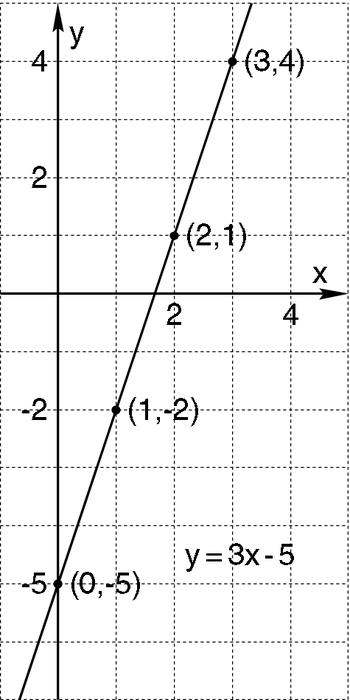
\includegraphics[width=0.2\textwidth]{fig32}
    \caption{Figur 3.2}
    \label{fig32}
\end{figure}

Hældningen er illustreret på figur 3.3. Hvis $x$ vokser til $x+1$, så vokser
$y$ fra $y_1$ til $y_2$ og forskellen $y_2-y_1$ er netop $a$. Bemærk, at $a$
også kan være negativ, nemlig når $y$ falder i værdi, når $x$ vokser.

\begin{figure}[ht]
    \centering
    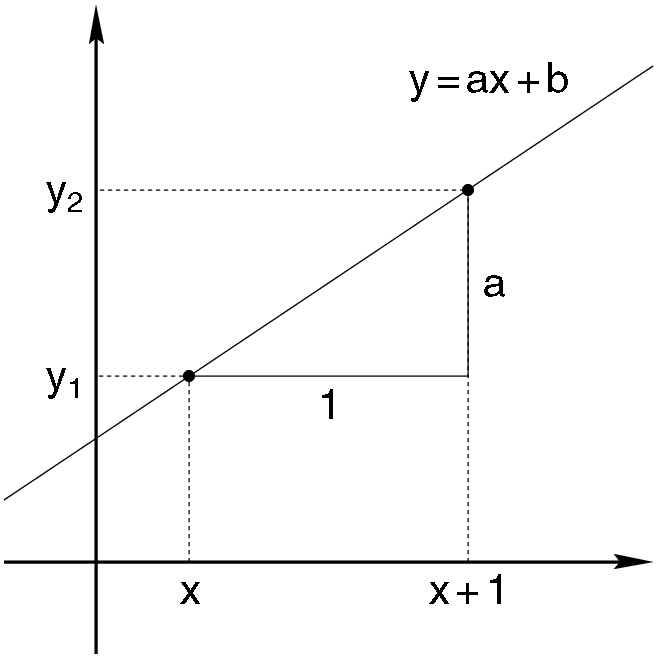
\includegraphics[width=0.5\textwidth]{fig33}
    \caption{Figur 3.3}
    \label{fig33}
\end{figure}

Linjer med samme hældning er parallelle. Linjer med positiv hældning forløber
opad mod højre, linjer med negativ hældning nedad mod højre. Linjer med
hældning 0 er vandrette.  Sådanne linjer har en ligning af formen $y=0x+b$
eller blot $y=b$.

At tallet $b$ er linjens skæringspunkt med $y$-aksen følger af, at
koordinatsættet $(0,\,b)$ passer i ligningen
$$
b = 0\cdot x+b
$$

\section{Ligefrem proportionalitet (kopi af afsnit i Mat-C bogen)}
Man bruger den talemåde, at to variabler $x$ og $y$ er {\em ligefrem
proportionale} (eller blot: proportionale), hvis de "stiger og falder i samme
takt". Vi skal se på, hvad denne lidt løse udtalelse dækker over.

Hvis en bil kører med konstant hastighed, f.eks. 90 km/t, kan vi opstille en
tabel over sammenhængen mellem tiden $x$ og den tilbagelagte afstand $y$:
$$
\begin{tabular}{c|c|c|c|c|c|c}
    x ({\rm min}) & 10 & 20 & 30 & 40 & 60 & 120 \\
    \hline
    y ({\rm km})  & 15 & 30 & 45 & 60 & 90 & 180  
\end{tabular}
$$
Vi ser, at $y$ netop er $1,5$ gange så stor som $x$, så sammenhængen mellem $x$
og $y$ kan udtrykkes som
$$
y = 1,5\cdot x
$$
Talemåden "$y$ ændrer sig i samme takt som $x$" betyder netop, at $x$ skal
ganges med et fast tal (her $1,5$) for at give $y$. Man kan også udtrykke det
sådan:
\begin{itemize}
    \item Når $x$ bliver dobbelt så stor, bliver $y$ også dobbelt så stor.
    \item Når $x$ bliver tre gange så stor, bliver $y$ også tre gange så stor.
    \item osv.
\end{itemize}
Hvis man med konstant hastighed kører dobbelt så lang tid, tilbagelægger man
også dobbelt så lang afstand, se figur 3.6.

\begin{figure}[ht]
    \centering
    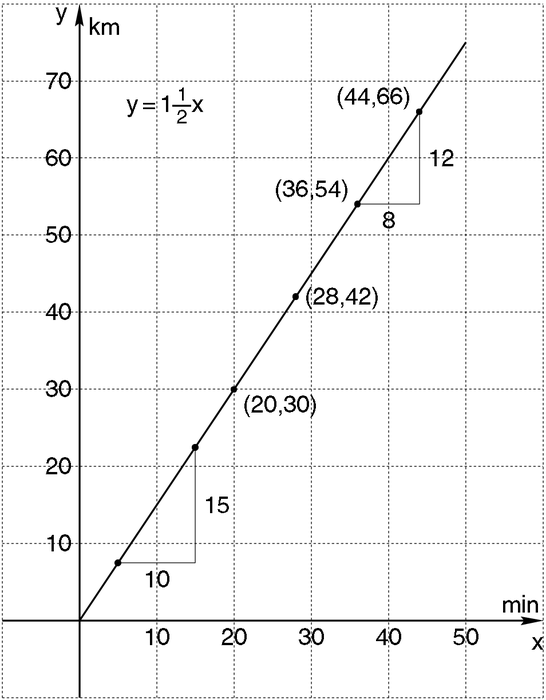
\includegraphics[width=0.5\textwidth]{fig36}
    \caption{Figur 3.6}
    \label{fig36}
\end{figure}

I dette tilfælde er tidsrummet $x$ og afstanden $y$ proportionale, og tallet
$1,5$ kaldes proportionalitetsfaktoren, fordi det netop er en faktor foran $x$.

Man kan også sige, at forholdet mellem $y$ og $x$ er konstant, fordi vi får:
$$
y = 1,5\cdot x \, \Leftrightarrow \, \frac{y}{x} = 1,5
$$
Forholdet mellem afstand og tid kaldes hastighed, og tallet angiver her netop
hastigheden: bilen kører med en hastighed på $1,5$ km/min, svarende til $90$
km/t.

Sammenhængen illustreres som en ret linje gennem $(0,\,0)$ med hældningen $1,5$.

\begin{mydef}
    To variabler $x$ og $y$ kaldes proportionale, hvis der findes et tal $k$, så
    $$
    y = k\cdot x \,\, {\rm eller} \,\, \frac{y}{x} = k
    $$
    Tallet $k$ kaldes proportionalitetsfaktoren. Sammenhængen mellem $x$ og $y$
    illustreres i koordinatsystemet af en ret linje gennem $(0,\,0)$ med 
    hældning $k$.
\end{mydef}

\subsection{Eksempel (sammenhæng mellem masse og volumen)}

Et eksempel på ligefrem proportionalitet er sammenhængen mellem masse og rumfang af olie.
Der gælder nemlig, at en liter olie vejer ca. 0,8 kg. To liter olie vejer derfor ca. 1,6 kg,
og generelt $x$ liter olie vejer $y$ kg, hvor
$$
y = 0,8 \cdot x
$$
Tallet $0,8$ er således vægten af én liter olie og det kaldes for olieets massefylde eller densitet.
At olie flyder oven på vand skyldes netop, at densiteten af olie er mindre end vands densitet.

\subsection{Eksempel (kopi af eksempel 3.4)}
I eksempel 1.1 så vi på teleselskabet, hvor prisen $y$ (naturligvis) afhænger af
taletiden $x$ i minutter:
$$
y=20+0,5x
$$
Her er prisen ikke proportional med taletiden: Dobbelt så lang taletid koster ikke
det dobbelte:
\begin{itemize}
    \item 15 minutter koster $20+0,5\cdot 15 = 27,50$ kroner.
    \item 30 minutter koster $20+0,5\cdot 30 = 35,00$ kroner.
\end{itemize}
I koordinatsystemet går linjen med ligningen $y=20+0,5x$ nemlig ikke gennem (0, 0),
sådan som kravet til proportionalitet er.

\section{Linje gennem to punkter -- omskrevet fra tilsvarende afsnit i Mat-C bogen}
Vi vil bestemme hældningen for en linje, der går gennem
to punkter med kendte koordinater. Vi viser følgende sætning:
\begin{thm}
    Hvis $A(x_1,\,y_1)$ og $B(x_2,\,y_2)$ er to punkter på en ret linje, der ikke
    er lodret, er hældningen $a$ bestemt ved
    $$
    a = \frac{y_2-y_1}{x_2-x_1}
    $$
\end{thm}
\begin{proof}
    Linjens ligning er 
    $$
    y = a\cdot x + b
    $$
    og netop de punkter, som ligger på linjen, har koordinater, der passer i
    ligningen.  Da $A$ og $B$ ligger på linjen, passer deres koordinater altså
    i ligningen, dvs.
    $$
    y_1 = a\cdot x_1 + b \,\, {\rm og} \,\, y_2 = a\cdot x_2 + b 
    $$
    Vi trækker den første ligning fra den sidste og får
    \bas
    y_2 - y_1 &=& a\cdot x_2 + b - (a\cdot x_1 + b) \\
              &=& a\cdot x_2 - a\cdot x_1 \\
              &=& a\cdot \left(x_2-x_1\right) 
    \eas
    altså
    $$
    a = \frac{y_2-y_1}{x_2-x_1}
    $$
    og det var netop, hvad vi ville vise.
\end{proof}

Læg mærke til, at vi i den sidste ligning har divideret med tallet $x_2-x_1$ på
begge sider af lighedstegnet. Dette tal er nemlig ikke $0$, fordi $x_1$ og
$x_2$ er forskellige tal -- vi har jo netop forudsat, at linjen ikke er lodret.

I formlen for hældningen $a$ angiver tælleren $y_2-y_1$ den lodrette afstand
mellem punkterne $A$ og $B$, mens nævneren $x_2-x_1$ angiver den vandrette
afstand. Vi kan derfor lidt populært sige, at
$$
a = \pm \frac{\mbox{lodret afstand}}{\mbox{vandret afstand}}
$$
Her står $\pm$ for at minde om, at der skal anbringes et minus foran brøken,
hvis hældningen er negativ.
\begin{eks}
    Vi ser på linjen $l$ gennem $A(-1,\,3)$ og $B(4,\,5)$.
    Linjens hældning er
    $$
    a = \frac{5-3}{4-(-1)} = \frac{2}{5} = 0,4
    $$
\end{eks}

Når man har beregnet hældningen $a$ så vil man også gerne bestemme skæringen
$b$.
\begin{thm}
    Hvis $A(x_1,\,y_1)$ er et punkt på en ret linje, og linjen har hældningen
    $a$, så er skæringen $b$ bestemt ved
    $$
    b = y_1 - a\cdot x_1
    $$
\end{thm}
\begin{proof}
    Linjens ligning er 
    $$
    y = a\cdot x + b
    $$
    og netop de punkter, som ligger på linjen, har koordinater, der passer i
    ligningen.  Da $A$ ligger på linjen, passer dens koordinater altså i
    ligningen, dvs.
    $$
    y_1 = a\cdot x_1 + b 
    $$
    Heri isoleres $b$:
    $$
    b = y_1 - a\cdot x_1
    $$
Dermed har vi vist det ønskede.
\end{proof}

\begin{thm}
    Hvis $A(x_1,\,y_1)$ er et punkt på en ret linje, og linjen har hældningen
    $a$, så er linjens lignign givet ved
    $$
    y = a\cdot (x-x_1) + y_1 
    $$
\end{thm}
\begin{proof}
    Vi indsætter resultatet fra sætning 4.3 i linjens ligning:
\bas
y &=& a\cdot x + (y_1 - a\cdot x_1) \\
  &=& a\cdot (x-x_1) + y_1 
\eas
Dermed har vi vist det ønskede.
\end{proof}


\section{Løse førstegradsligninger (kopi af afsnittet ligninger fra Mat-A1 bogen)}
En ligning er af første grad, hvis den er af typen
$$
ax + b = 0\; ,
$$
eller umiddelbart kan omskrives til en sådan ligning. Her er et par eksempler:
$$
3x - 4 = 8 + 2x \quad , \quad 5(x - 4) + 2x = 6x - 2(3 - 4x)\; .
$$

\subsection{Ensbetydende ligninger}
Hvis man foretager en række omformninger af en ligning for at finde en løsning,
bruger man symbolet $\iff$ , en dobbeltpil (eller en biimplikation), mellem
ligninger, der har de samme løsninger. Fx har vi
\bas
&& 2(3x - 1) = x - 4(2 - x)\\
&\iff& 6x - 2 = x - 8 + 4x\\
&\iff& 6x - 2 = 5x - 8 \\
&\iff& x = -6 
\eas
Hver af de fire ligninger har den samme løsning. Man siger, at sådanne
ligninger er ensbetydende. Man kan også sige, at ensbetydende ligninger fremgår
af hinanden ved ’lovlige’ omformninger.

Vi anfører de vigtigste regler for løsning af ligninger.

[ANIMATION OM REGNEREGLER 1--4]


\section{Skæring mellem linjer -- omskrevet fra tilsvarende afsnit i Mat-C bogen}
Hvis to linjers ligninger er kendt, vil vi finde koordinaterne til linjernes
skæringspunkt (hvis de ikke er parallelle).

Linjerne $l$ og $m$ har f.eks. ligningerne (se figur xx)
$$
l: y=0,5x-2\,\,{\mbox{og}}\,\,m: y=-3x+5
$$

\begin{figure}[ht]
    \centering
    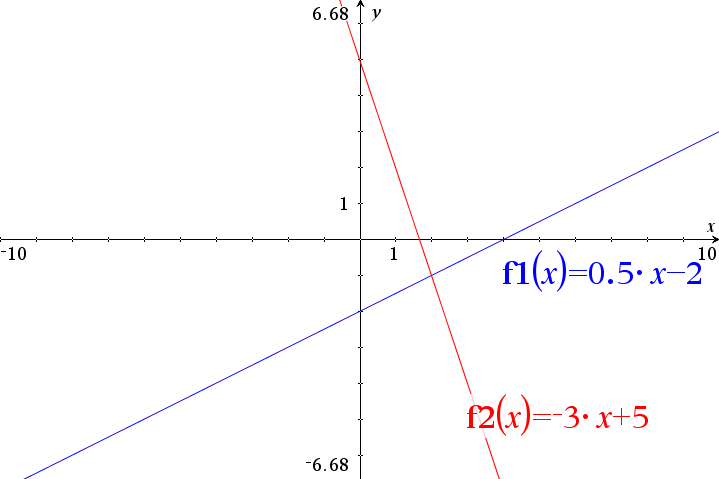
\includegraphics[width=0.5\textwidth]{fig6}
    \caption{Figur 6}
    \label{fig6}
\end{figure}

I skæringspunktet mellem linjerne skal $y$-værdien for de to linjer være den
samme, så der må gælde, at
$$
0,5x-2 = -3x+5
$$
og denne ligning løses på følgende måde:
\bas
&& 0,5x+3x=5+2\\
&\iff& 3,5x=7\\
&\iff& x=2
\eas
Denne værdi af $x$ indsættes i en af ligningerne, ligegyldig hvilken:
$$
y=0,5\cdot2-2=-1
$$
Skæringspunktet har altså koordinaterne $(2,\,1)$, hvilket ser ud til at
stemme med figuren.

\section{Lineær regression -- kopi af afsnit i Mat-A2 bogen}
På fig. 5.4 er afsat punkterne med koordinaterne (1, 2), (2, 5), (3, 6) og (4,
7). De ligger ikke på ret linje, men med tilnærmelse ligger de på linjen med
ligningen y = 1,6x + 1.

\begin{figure}[ht]
    \centering
    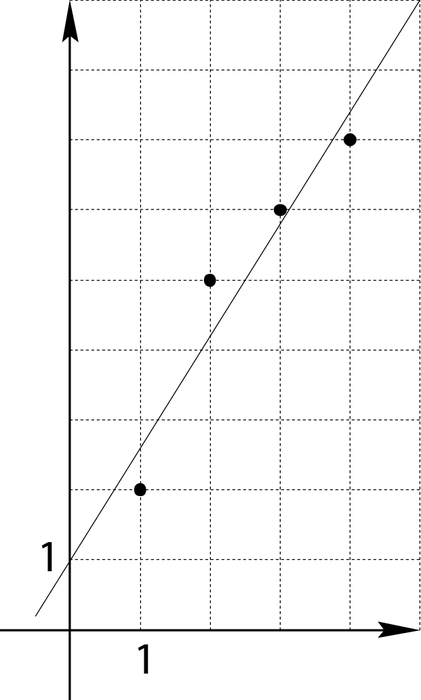
\includegraphics[width=0.5\textwidth]{fig54}
    \caption{Figur 5.4}
    \label{fig54}
\end{figure}

Men er dette nu den 'nøjagtigste' linje? Skulle vi måske hellere have valgt
linjen y = 1,65x + 0,97 eller y = 1,58x + 1,04 eller ...?

Man benytter sædvanligvis ved tilnærmelse med rette linjer til givne
målepunkter en metode, der kaldes de mindste kvadraters metode.

\begin{figure}[ht]
    \centering
    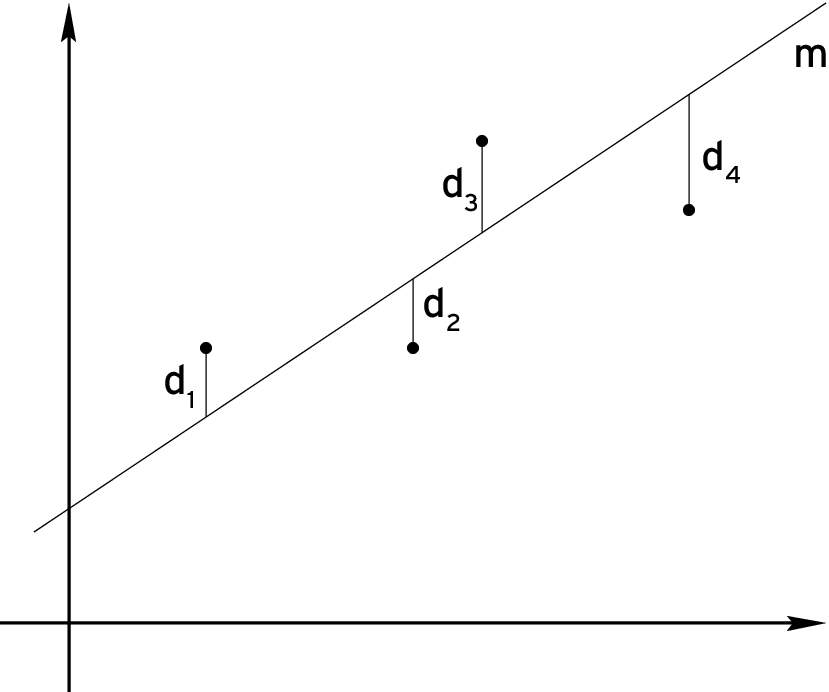
\includegraphics[width=0.5\textwidth]{fig55}
    \caption{Figur 5.5}
    \label{fig55}
\end{figure}

På fig. 5.5 er en række punkter afsat, og linjen m er tegnet. Desuden er de
lodrette afstande $d_1$, $d_2$, $d_3$, ..., $d_n$ fra målepunkterne til linjen afsat. Man
kan så udregne summen $D$ af kvadraterne (kvadratsummen) på afstandene:

$$
D = {d_1}^2 + {d_2}^2 + {d_3}^2 + \ldots + {d_n}^2 \; . 
$$

Hvis man vælger en anden linje, får man selvfølgelig i reglen en anden kvadratsum.

Man har vedtaget at den linje, der gør kvadratsummen $D$ mindst mulig, er den
'bedste' linje. Metoden kaldes de mindste kvadraters metode, og den linje, der
fremkommer, kaldes regressionslinjen svarende til punkterne. Vi går ikke ind
på, hvordan linjen matematisk bestemmes. 


Man har undersøgt højden af et stort antal piger og beregnet middelhøjden for
hver årgang. Pigernes højde ved forskellige aldre fremgår af skemaet.

\begin{tabular}{c|c|c|c|c|c|c|c}
    Alder (år), x &  2 &  3 &  4 &  5 &  6 &  7 &  8 \\
    Højde (cm), y &  89,2 &   98,3 &   104,9 &  112,0 &  118,1 &  123,4 &  131,3
\end{tabular}

\begin{tabular}{c|c|c|c|c|c|c}
    Alder (år), x  & 9  & 10 & 11&  12 & 13 & 14 \\
    Højde (cm), y  & 136,4 &  142,5 &  151,1 &  155,4 &  159,8 &  161,5
\end{tabular}

Det ser ud til, at højden øges med ca. 6 cm, når alderen øges med 1 år, så det
er rimeligt at forvente en lineær sammenhæng.

Ved hjælp af CAS kan vi finde ligningen for regressionslinjen til

$$
y = 6,17x + 80,19 \; .
$$

\begin{figure}[ht]
    \centering
    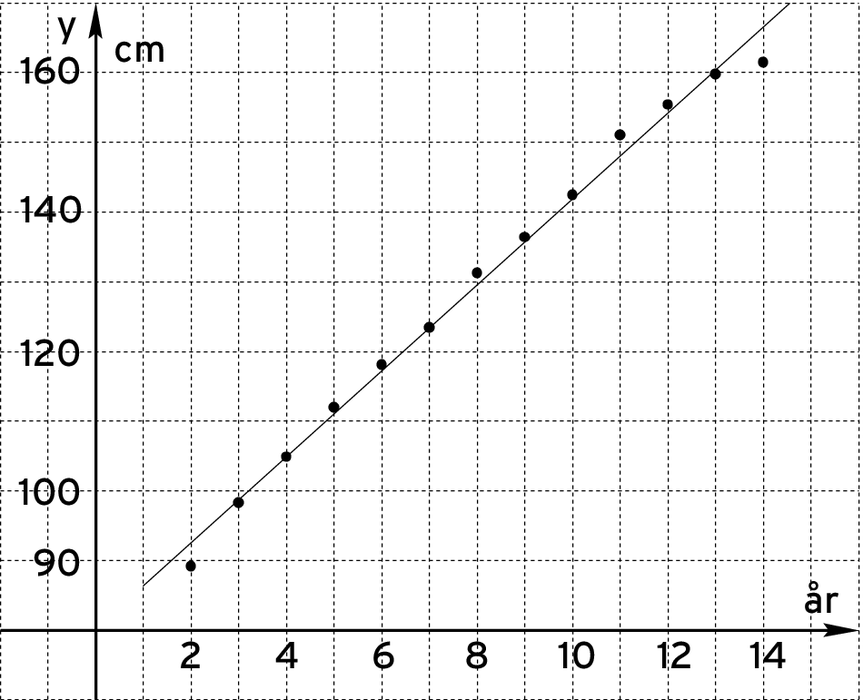
\includegraphics[width=0.5\textwidth]{fig56}
    \caption{Figur 5.6}
    \label{fig56}
\end{figure}

Den gennemsnitlige vækst i pigernes højde er altså 6,17 cm pr. år. På fig. 5.6
ses et diagram over pigernes højder med regressionslinjen indtegnet.

\subsection{Korrelation}
CAS giver foruden regressionslinjens ligning den såkaldte
korrelations\-koef\-fi\-cient $r$. Vi kommer ikke her ind på teorien bag beregningen af
dette tal, men nøjes med at bemærke, at korrelationskoefficienten er et mål for
den lineære sammenhæng mellem punkterne.

Vi bemærker følgende om korrelationskoefficienten r:

\begin{itemize}
    \item Hvis $r = 1$ ligger punkterne præcis på ret linje med positiv hældning.
    \item Hvis $0 < r < 1$ har regressionslinjen positiv hældning. Jo tættere $r$
        er på 1, desto tættere ligger punkterne på linjen.
    \item Hvis $r = 0$ eller tæt ved 0, er der ingen eller kun svag lineær sammenhæng.
    \item Hvis $-1 < r < 0$ har regressionslinjen negativ hældning. Jo tættere $r$
        er på -1, desto tættere ligger punkterne på linjen.
    \item Hvis $r = -1$ ligger punkterne præcis på ret linje med negativ hældning. 
\end{itemize}
På fig. 5.7 er disse forhold illustreret.

\begin{figure}[ht]
    \centering
    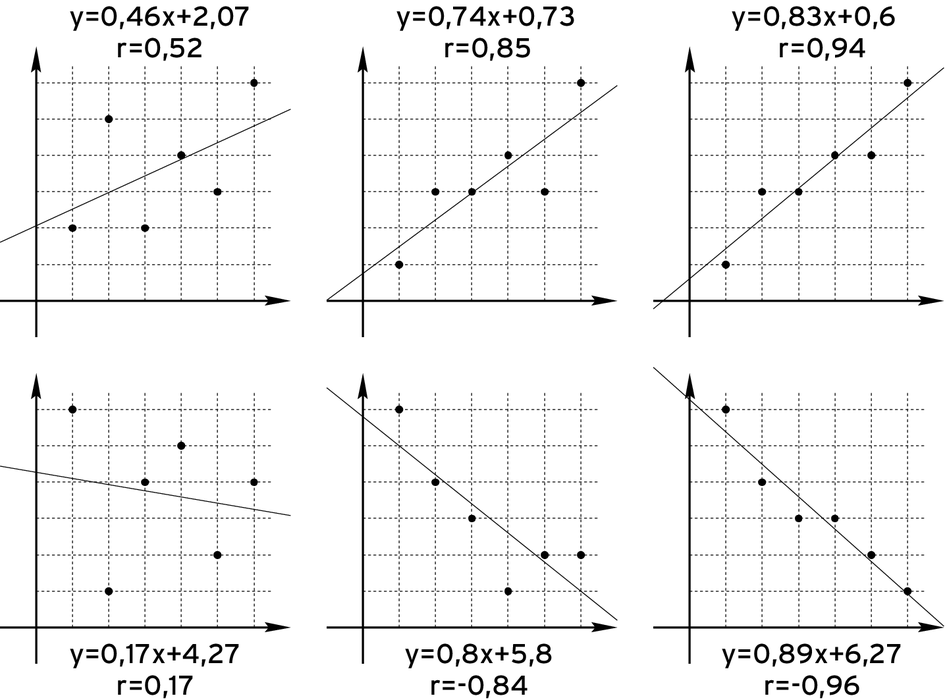
\includegraphics[width=0.5\textwidth]{fig57}
    \caption{Figur 5.7}
    \label{fig57}
\end{figure}


\section{Intervaller -- kopi af afsnit fra Mat-A1 bogen}

Vi kender den sædvanlige tallinje med begyndelsespunkt O og det såkaldte
enhedspunkt E, der svarer til tallet 1. Længden af linjestykket OE er altså 1.

\begin{figure}[ht]
    \centering
    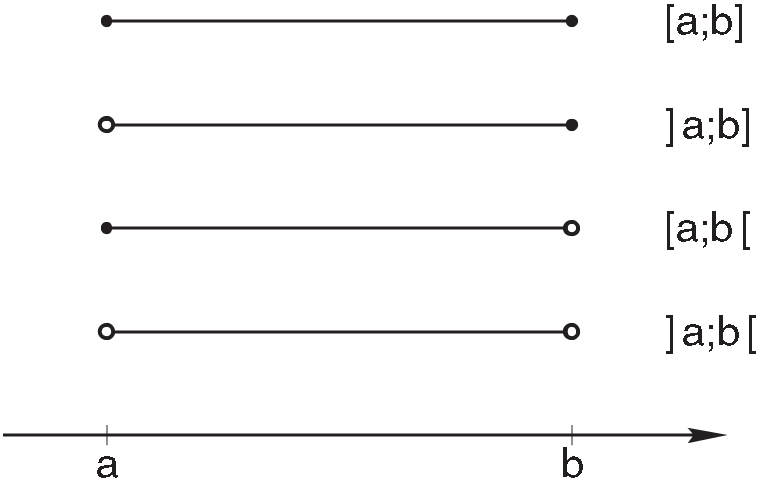
\includegraphics[width=0.5\textwidth]{fig23}
    \caption{Figur 2.3}
    \label{fig23}
\end{figure}

Vi ser på visse dele af tallinjen, de såkaldte intervaller.

\subsection{Begrænsede intervaller}
Hvis a og b er to tal, så a < b, skriver vi (se fig. 2.3):
\begin{itemize}
    \item $[a;b]$ : alle tal mellem a og b, a og b medregnet,
    \item $[a;b[$ : alle tal fra og med a til, men ikke med b,
    \item $]a;b]$ : alle tal fra a til b, men ikke med a,
    \item $]a;b[$ : alle tal mellem a og b, a og b ikke medregnet .
\end{itemize}
Disse afsnit af tallinjen kaldes intervaller, og a og b er deres endepunkter.

Vi siger, at et interval er
\begin{itemize}
    \item lukket, hvis begge endepunkter er med i intervallet,
    \item halvåbent, hvis det ene, men ikke det andet endepunkt er med i intervallet,
    \item åbent, hvis ingen af endepunkterne er med i intervallet.
\end{itemize}
Intervaller af disse fire typer er alle begrænsede, og deres længde er $b-a$.

\begin{eks}
Intervallet $[3;7[$ består af alle tal på tallinjen mellem 3 og 7; 3 er
medregnet og 7 er ikke medregnet. Intervallets længde er $7-3 = 4$ .

Intervallet $[-5;8]$ består af alle tal mellem -5 og 8, og både -5 og 8
tilhører intervallet. Dets længde er 13 fordi $8 - (-5) = 13$ .

På tallinjen er et intervals længde altså afstanden mellem endepunkterne.
\end{eks}

\subsection{Ubegrænsede intervaller}
Vi får tit brug for at se på tal, der på tallinjen ligger til højre eller til
venstre for et givet tal (fig. 2.4), fx alle tal der er større end 17, eller
alle tal der er mindre end eller lig med 50.

Det giver anledning til disse skrivemåder:

\begin{itemize}
    \item $[a;\infty[$  : alle tal større end eller lig med a
    \item $]a;\infty[$  : alle tal større end a
    \item $]-\infty;b]$ : alle tal mindre end eller lig med b
    \item $]-\infty;b[$ : alle tal mindre end b
\end{itemize}
Tegnet $\infty$ læses ’uendelig’.

Intervallerne af typerne $]a;\infty [$ og $]-\infty ;b[$ kaldes åbne, da a og b
ikke medregnes, og intervallerne af typerne $[a;\infty [$ og $]-\infty ;b]$
kaldes lukkede, da a og b medregnes.

Disse intervaller er ubegrænsede, fordi de ikke har nogen længde – det
fortsætter ’i det uendelige’ i den ene ende af tallinjen.

Endelig kan man også skrive intervallet $]-\infty ;\infty [$. Dette angiver
alle tal på tallinjen.

\section{Uligheder (kopi af Mat-B1 HTX)}
Vi har tidligere set på en række forskellige ligningstyper. Fælles for disse
ligninger er, at de alle indeholder et lighedstegn. Vi skal nu se på et emne,
der under ét benævnes uligheder. Uligheder optræder også i teknikkens verden.
Skibe, der skal kunne besejle Panama-kanalen, må højest være 32,3 meter bredde.

$$
B\leq 32,3 \, \text{m}
$$
Temperaturen skal være mindst $800^\circ$ i en given proces:


$$
T \geq 800 ^\circ C
$$
Som det ses, optræder der ulighedstegn. Dem findes der fire af, to skarpe og to svage:

\begin{itemize}
    \item Mindre end, (skarp) <
    \item Større end, (skarp) >
    \item Mindre end eller lig med, (svag) $\leq$
    \item Større end eller lig med, (svag) $\geq$
\end{itemize}

Et par eksempler på uligheder:

$$
x-2>7 \;\;\; \text{og} \;\;\; 3\cdot x-12\geq 4
$$

Når vi skal løse uligheder, er teknikken stort set den samme som ved ligninger, dog med en enkelt vigtig undtagelse.

Et led kan flyttes fra den ene side af ulighedstegnet til den anden side ved at skifte fortegn:
$$
x+3<7 \Leftrightarrow x<7-3 \Leftrightarrow x<4
$$
$$
13-x>3 \Leftrightarrow 13>3+x \Leftrightarrow 10>x
$$
Bemærk, at en ulighed kan læses fra to sider:
$10 < x$ er det samme som $x > 10$

Ved multiplikation og division skal vi være forsigtige. Det er tydeligt for enhver, at:
$$
2<7
$$
Vi ganger med et positivt tal på begge sider:
$$
3 \cdot 2 <3 \cdot 7 \Leftrightarrow 6<21
$$
Det gik fint.

Vi prøver at nu at gange med et negativt tal, her -1, på begge sider af ulighedstegnet:
$$
(-1) \cdot 2 < (-1) \cdot 7 \Leftrightarrow -2<-7
$$
Det går ikke! -2 er jo større end -7. Vi er åbenbart nødt til at vende ulighedstegnet om:
$$
2<7 \Leftrightarrow (-1) \cdot 2 > (-1) \cdot 7 \Leftrightarrow -2>-7
$$
Ud fra eksemplerne kan vi opstille følgende regler:
\begin{enumerate}
    \item Et led flyttes fra den ene side af ulighedstegnet til den anden side ved at skifte fortegn på leddet.
    \item Man må gange og dividere med det samme positive tal, undtagen 0, på begge sider af ulighedstegnet.
    \item Man må gange og dividere med det samme negative tal på begge sider af ulighedstegnet, hvis man samtidig vender ulighedstegnet om.
\end{enumerate}

\begin{eks}
Vi løser uligheden:
$$
3 \cdot x - 7 \geq 8
$$
Led kan flyttes som i ligninger:
$$
3 \cdot x \geq 8+7 \Leftrightarrow 3 \cdot x \geq 15
$$
Vi må gange og dividere med positive tal:
$$
3 \cdot x \geq 15 \Leftrightarrow x \geq 5
$$
\end{eks}

\begin{eks}
Vi løser denne ulighed:
$$
-4 \cdot x + 1 \leq 21
$$
Et led flyttes:
$$
-4 \cdot x \leq 21 -1 \Leftrightarrow -4 \cdot x \leq 20
$$
Nu skal vi passe på! Vi isolerer x ved at dividere med -4 på begge sider og skal huske at vende ulighedstegnet:
$$
-4 \cdot x \leq 20 \Leftrightarrow x \geq-5
$$

Vi kunne have grebet opgaven anderledes an:
$$
-4 \cdot x + 1 \leq 21
$$
$$
-4 \cdot x + 1 \leq 21 \Leftrightarrow 1 - 21 \leq 4 \cdot x
$$
Nu er koefficienten foran x positiv:
$$
1-21 \leq 4 \cdot x \Leftrightarrow -20 \leq 4 \cdot x \Leftrightarrow -5 \leq x
$$
Hvis vi læser løsningen ”baglæns” fås:
$$
x \geq -5
$$
Altså samme løsning som før. Heldigvis!
\end{eks}

\subsection{Dobbeltuligheder}
En ulighed med to ulighedstegn, der vender samme vej (hvorfor skal de vende samme vej?) kaldes for en dobbeltulighed:
$$
x-1 < 2x + 3 < x+11
$$

Den løses ved at opdele uligheden i to uligheder:
$$
x - 1 < 2x + 3 \;\;\; \text{og} \;\;\; 2x + 3 < x + 11
$$
der løses med den angivne metode, og hvor den endelige løsning skal opfylde begge kriterier. I det angivne tilfælde skal der gælde:
$$
x>-4 \;\;\; \text{og} \;\;\; x<8
$$
Og dermed skal der alt i alt gælde at
$$
-4 < x < 8
$$

\end{document}

